%%%%%%%%%%%%%%%%%%%%%%%%%%%%%%%%%%%%%%%%%%%%%%%%%%%%%%%%%%%%%%%%%%%%%%%%%%%%%%%%
%2345678901234567890123456789012345678901234567890123456789012345678901234567890
%        1         2         3         4         5         6         7         8

\documentclass[letterpaper, 10 pt, conference]{ieeeconf}  % Comment this line out if you need a4paper

%\documentclass[a4paper, 10pt, conference]{ieeeconf}      % Use this line for a4 paper

\IEEEoverridecommandlockouts                              % This command is only needed if 
                                                          % you want to use the \thanks command

\overrideIEEEmargins                                      % Needed to meet printer requirements.

% See the \addtolength command later in the file to balance the column lengths
% on the last page of the document

% The following packages can be found on http:\\www.ctan.org
\usepackage{graphics} % for pdf, bitmapped graphics files
\usepackage{epsfig} % for postscript graphics files
%\usepackage{mathptmx} % assumes new font selection scheme installed
%\usepackage{times} % assumes new font selection scheme installed
%\usepackage{amsmath} % assumes amsmath package installed
%\usepackage{amssymb}  % assumes amsmath package installed
\usepackage{booktabs}

\title{\LARGE \bf
Soft Wearable Augmented Walking Suit with Pneumatic Gel Muscles and Stance Phase Detection System to Assist Gait
}



\author{Chetan Thakur$^{1}$ Kazunori Ogawa$^{1,2}$ Toshio Tsuji$^{1}$ Yuichi Kurita$^{1}$% <-this % stops a space
\thanks{*The author (Chetan Thakur) was supported through the Hiroshima University
TAOYAKA Program for creating a flexible, enduring, peaceful society, funded by the Program for Leading
Graduate Schools, Ministry of Education, Culture, Sports, Science and Technology.}% <-this % stops a space
\thanks{$^{1}$Department of Systems Cybernetics, Graduate School of Engineering,
	Hiroshima University, Hiroshima, Japan
        {\tt\small }}%
\thanks{$^{2}$Daiya Industries Co. Ltd. Japan
        {\tt\small }}%
}


\begin{document}
\special{papersize=8.5in,11in}
\setlength{\pdfpageheight}{11in}
\setlength{\pdfpagewidth}{8.5in}

\maketitle
\thispagestyle{empty}
\pagestyle{empty}

\maketitle
\thispagestyle{empty}
\pagestyle{empty}


%%%%%%%%%%%%%%%%%%%%%%%%%%%%%%%%%%%%%%%%%%%%%%%%%%%%%%%%%%%%%%%%%%%%%%%%%%%%%%%%
\begin{abstract}

Lower limb of human body is responsible for human locomotion and maintain good quality of life. But there are many cases of muscle fatigue or injuries due to stressful work environment, aging and work that involve walking long distance. Therefore, there is a need of walking assistive suit which can unload muscle activation during walking and reduce the chances of lower limb muscle fatigue. In this paper we discuss about development of lightweight and wearable Augmented Walking Suit using Pneumatic Gel Muscle and its actuation control using lower limb pose detection mechanism by taking human gait cycle in consideration. The objective of this assistive suit is to reduce required muscle effort of posterior and anterior muscle during swing phase of the gait cycle thereby making it easier to move forward. To evaluate the effects of the suit we tested this suit with random subjects and record surface EMG (sEMG) of 8 major lower limb muscles for three level of assistive forces. The evaluation was done based on the sEMG signal envelope for each subject for different level of assistive forces and statistical difference in \%MVC of 8 major lower limb muscles active during gait cycle. In our result we found that all subjects showed no change or a statistically significant reduction in muscle efforts due to assistive suit for all the muscles responsible for swing phase of the gait cycle. 
\end{abstract}


%%%%%%%%%%%%%%%%%%%%%%%%%%%%%%%%%%%%%%%%%%%%%%%%%%%%%%%%%%%%%%%%%%%%%%%%%%%%%%%%
\section{INTRODUCTION}
Ability to move uninterrupted is one of the critical function of human body. It is one of the reasons for enjoying a good quality of life by enabling one to be independent for performing a variety of daily tasks. However, there are many instances such as aging, accidents and longer and more stressful working conditions that result in muscle fatigue and injuries making it difficult to walk by affecting the quality of life of the individual. Such situation can be avoided or addressed using exoskeletons or wearable assistive devices. Muscle activation pattern of human gait is dynamic, and changes as the motion or intent are changed, but the basic pattern of gait cycle is same for all. While developing AWS we considered factors such as nature of work area, age, flexibility to use in outside environment, lightweight, portable, easy to use, reduces muscle efforts during walking and no impact on normal gait cycle. With increasing elderly population, stressful work condition devices like these will play a significant role in improving the quality of life. L. Garçon et al. \cite{1} in his review mentioned there are large requirement assistive devices for mobility for people such as elderly, disabled and healthcare staff for various tasks involved in daily life. Among various lower limb assistive devices, there exists tradeoff between autonomous actuation, wearable, lightweight and affordability. HAL \cite{2} which enable walking easier for elderly and rehabilitation post stroke or accidents. Wearable agri robot \cite{3} designed for supporting farming activities and reduce muscle fatigue, it supports body posture and reduces the muscle fatigue. Walking assist device with body weight support system \cite{4} for augmenting walking and assistive squats motion required for pick and place tasks in the various work environment. RoboKnee \cite{5} is one DOF exoskeleton designed to support human locomotion such as walk and stair climbing. Plantarflexion assist exoskeleton \cite{6} is designed to reduce the metabolic cost of walking. 

These devices are divided into segments such as healthcare, disability support and augmenting locomotion. These devices augment human motion significantly, but its use in outside environment is limited especially in agriculture and factory settings. For augmented walking wearable, lightweight, portable, easy to use and reduce muscle fatigue, these criteria are essential and together missing in assistive devices discussed above. To solve this problem previously, we developed a lightweight, low powered pneumatic gel muscle (PGM) \cite{7} as shown in Fig \ref{fig:pgm}. PGM can generate force with 60 kPa air pressure which is not possible in McKibben pneumatic artificial muscle (PAM) \cite{8}. It is also structure in a way to be stitched to fabric or fix using velcro tapes; this makes it easy to design the assistive suit. Fig \ref{fig:pgmelongationratio} shows the relation of supplied air pressure, generated force and maximum elongation as a percentage of resting length.

In \cite{9} we devised the concept if Unplugged Powered Suit for walking assist using the advantage of PGM and gait cycle. The actuation control of PGM was designed by attaching pump at the heel of a shoe. This configuration was able to generate minimal assistive force for walking. However, the challenge of this configuration changes in shoe design and placement of pumps in the shoe for generation of assistive force. 

In this paper, we discuss the design and control of AWS, which improves on Unplugged Powered Suit (UPS) by keeping human gait in the loop by using gait cycle identification system for generating assistive force. In section \ref{methodology} PGM and its force characteristics, biomechanics and human gait detection system and design and configuration of the Augmented walking suit is discussed. In section \ref{Evaluation}, we discuss the evaluation criteria, experiment method setups, results of the lower limb surface EMG (sEMG) evaluation for two levels of assistive force with the comparison of average gait sEMG envelope for all subjects and statistical analysis. Section \ref{discuss} presents the discussion, conclusion and future works.


\section{Methodology} \label{methodology}

\subsection{Pneumatic Gel Muscle} \label{pgm}
\begin{figure}
	\centering
	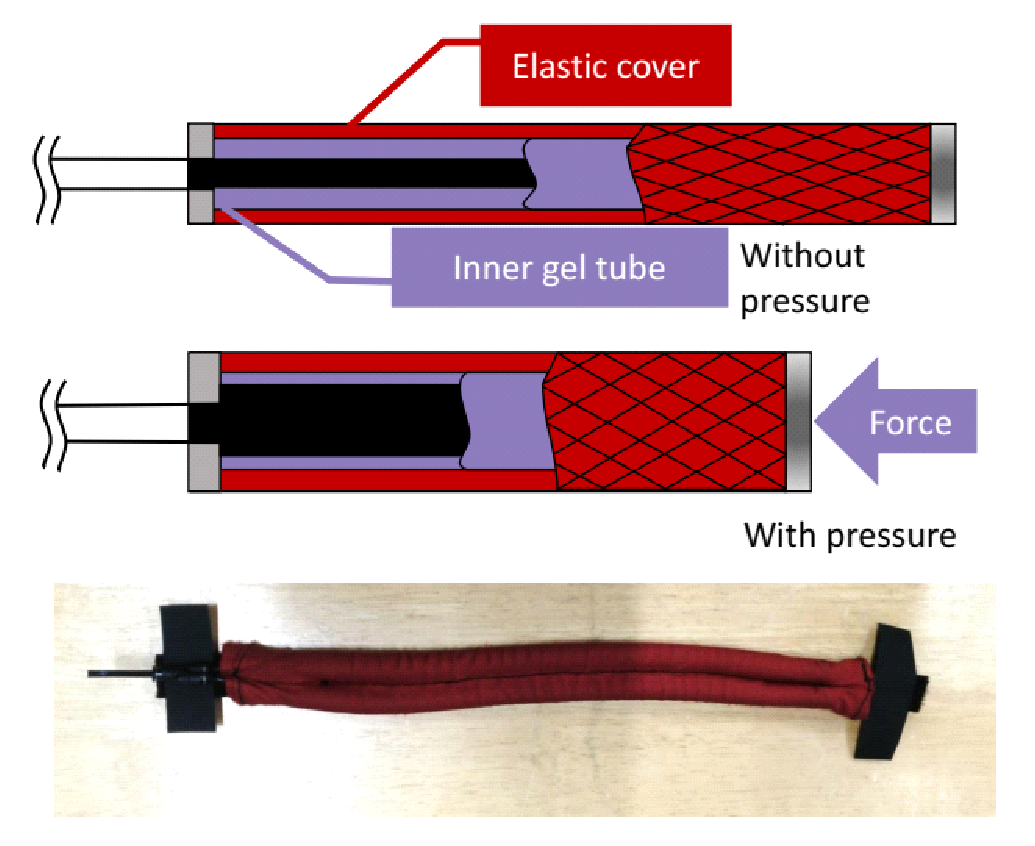
\includegraphics[width=0.5\linewidth]{../photos/pgm}
	\caption{Pneumatic Gel Muscle schematic Diagram and Real Product}
	\label{fig:pgm}
\end{figure}
\begin{figure}
	\centering
	\includegraphics[width=0.9\linewidth, height=0.2\textheight]{../photos/PGMelongationratio}
	\caption{Pneumatic Gel Muscle's elongation and force generation characteristics \cite{7}}
	\label{fig:pgmelongationratio}
\end{figure}

PGM is a special type of PAM designed to be driven by low air pressure. Figure 1 shows schematics and real prototype of the PGM. It has resting length of 30 cm, maximum contraction length of 25 cm and maximum elongation length of 45 cm. Construction of PGM includes inner tube made of special styrene-based thermoplastic elastomer to improve the flexibility and outer protective mesh. Traditional PAM have rubber or silicon based rubber tubes covered with protective mesh, these tubes need more air pressure to inflate whereas in case of PGM can generate force with air pressure as low as 50 kPa up to 300 kPa as reported by [7]. The flexible design and working with low air pressure makes it more suitable choice for development of wearable assistive suits as compared to traditional PAM who have higher force generating capacity but requires larger air pressure. Figure \ref{fig:pgmelongationratio} shows elongation ratio of the PGM as measured by \cite{7} it shows force generating capacity of the PGM and elongation length for various level of air pressure. In the experiment the one end of PGM is fixed and test load is added to other end to. Whereas in AWS both end of the PGM are fixed and stretched, in this case the force generating capacity of the PGM changes. This change is not measure in \cite{7}, therefore we conducted an experiment to measure force generated by PGM for stretched and un-stretched condition and different air pressure. The supported range of air pressure is 50 kPa to 300 kPa. Fig \ref{fig:pgmtest} show experiment setup, where one end is connected to load cell and at the other end air source is connected through Panasonic ADP5161 air pressure sensor. Experiment is conducted for two cases unstretched and stretched to 45 cm. Figure 3 shows the measured force profile for two conditions in both cases PG shows linear force generation characteristics which is modeled as linear equation as described in equation 1 and 2 with their respective $R^2$ values. These models exhibit similar force generating behavior when used in AWS configuration. These characteristics can be used for controlling assistive force generated by PGM when in AWS.

\begin{figure}
	\centering
	\includegraphics[width=0.7\linewidth]{../photos/pgmtestsetup}
	\caption{Force profile test setup}
	\label{fig:pgmtest}
\end{figure}

\begin{figure}
	\centering
	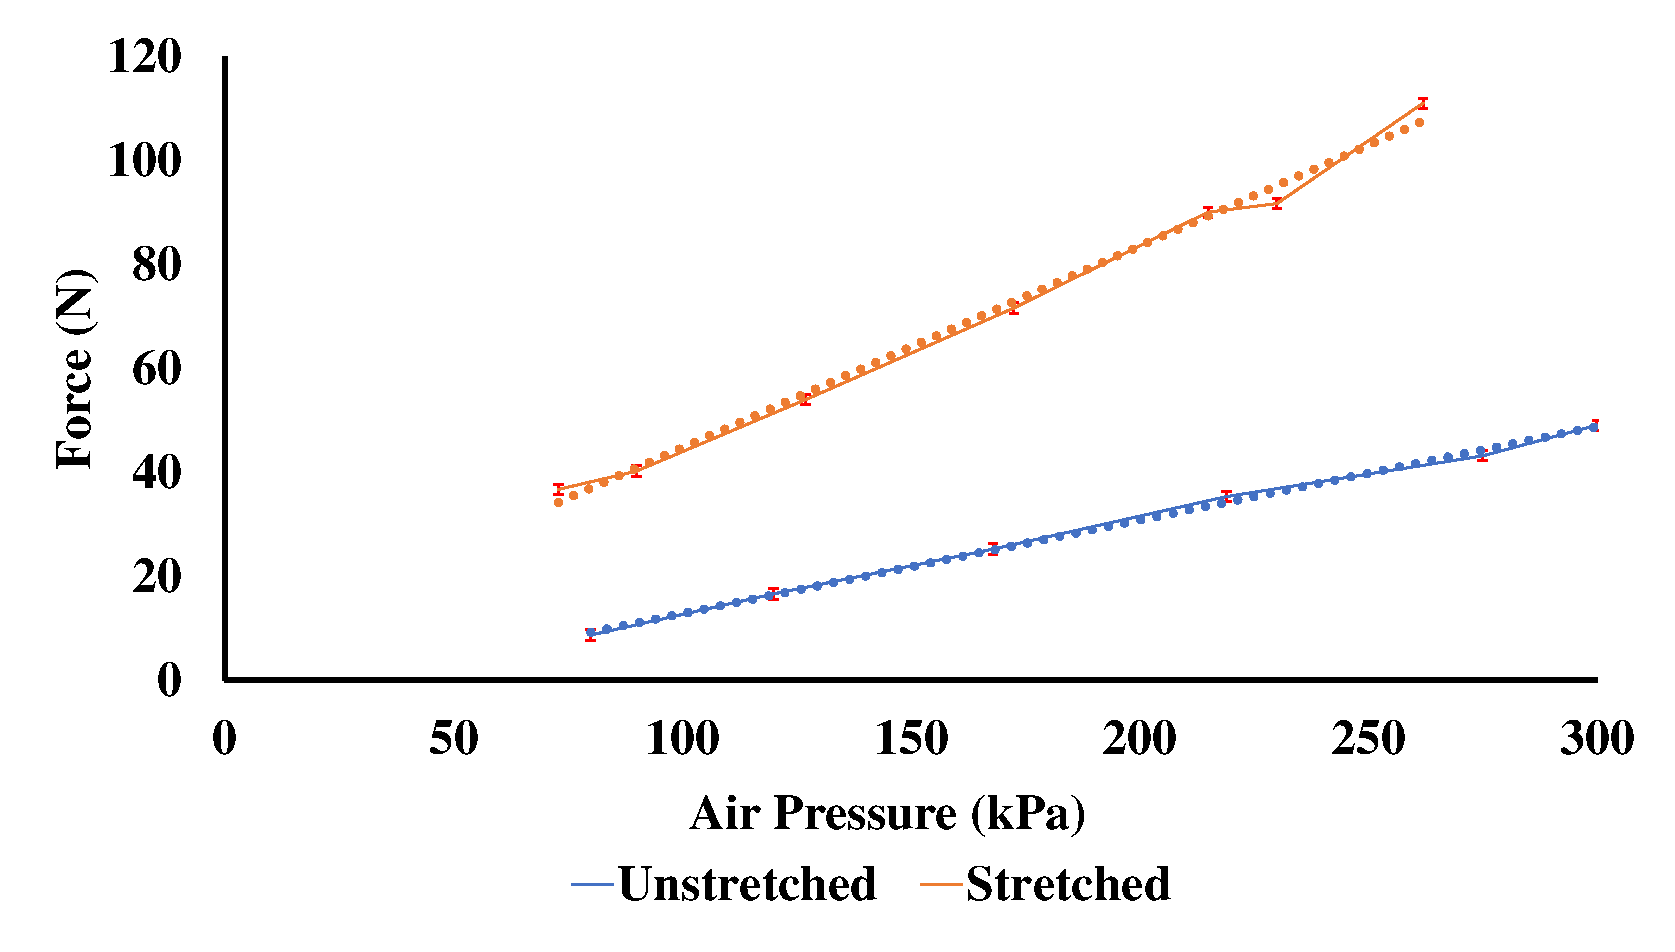
\includegraphics[width=0.9\linewidth]{../photos/PGMforceprofile}
	\caption{PGM force profile for unstretched and stretched condition}
	\label{fig:pgmforceprofile}
\end{figure}


\begin{equation}\label{pgmunstreched}
y=0.1799x - 5.1983; (R^2=0.993)
\end{equation}
\begin{equation}\label{pgmstreched}
y = 0.3883x + 5.8899; ; (R^2=0.9985)
\end{equation}

\subsection{Biomechanics of gait cycle } \label{gaitcycle}
The design and control of the AWS is based on human walking i.e. gait cycle and depends on how we walk. The gait cycle is divided into three major phases i.e. stance phase, double limb support phase and swing phase. The stance phase is responsible for weight acceptance and load transfer to support swing phase of the contralateral limb, Figure \ref{fig:gait} shows schematic block diagram of the gait cycle. In stance phase muscle activation of tibialis anterior (TA), quadriceps femoris i.e. rectus femoris (RF), vastus medialis (VM), vastus lateralis (VL), soleus (SOL), medial gastrocnemius (MG) and lateral gastrocnemius (LG) is observed. These muscles are responsible from heel strike till toe off in the stance phase. In the double limb support phase the limb going in stance phase support the forward locomotion of the contralateral limb going in swing phase. In this phase both the limbs are in the ground for about 10\% of the one gait cycle. In this phase SOL, LG, MG and RF muscles are active and responsible for the limb going in swing phase. In the swing phase limb makes forward movement and RF, VL, VM, biceps femoris (BF)  are major muscle contributors of this phase. 

Apart from the complex muscle activation foot position and orientation also changes. In stance phase foots orientation start from heel strike then flat foot, heels off and ends with toe off. We used this information to process and use it for gait detection and actuation control of the AWS suit. 

\begin{figure}
	\centering
	\includegraphics[width=0.8\linewidth]{../photos/gait}
	\caption{Gait Cycle Classification}
	\label{fig:gait}
\end{figure}


\subsection{AWS Design and Actuation Control Mechanism}

\begin{figure}
	\centering
	\includegraphics[width=0.7\linewidth]{../photos/aws}
	\caption{Augmented Walking Suit}
	\label{fig:aws}
\end{figure}


\begin{figure}
	\centering
	\includegraphics[width=1\linewidth,height=0.5\linewidth]{../photos/awscontrol}
	\caption{AWS Control mechanism}
	\label{fig:awssystem}
\end{figure}
\begin{figure}
	\centering
	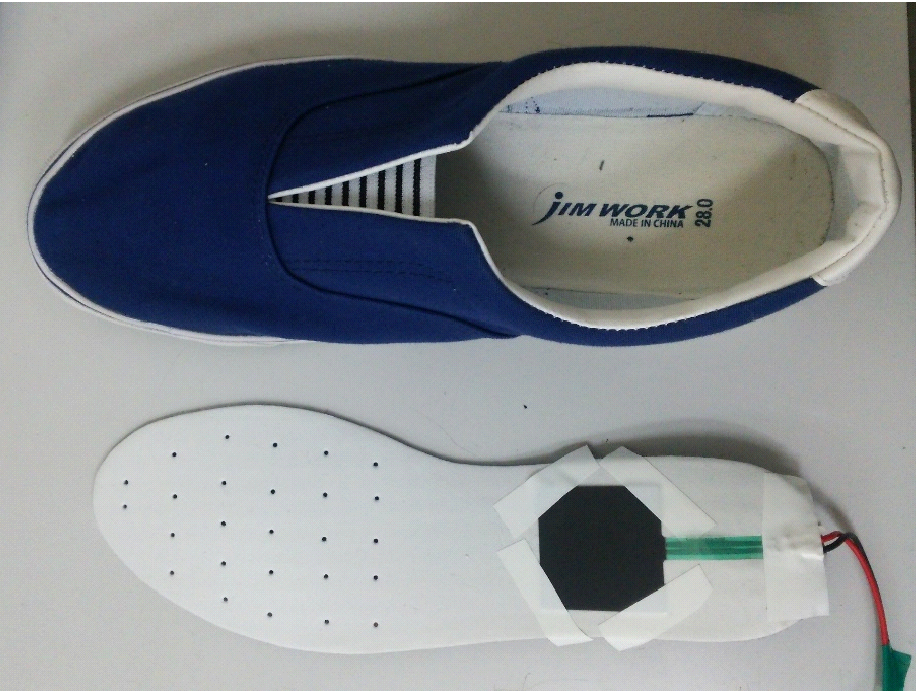
\includegraphics[width=4cm]{../photos/fsrsole}
	\caption{FSR-406 sensor placement in shoe}
	\label{fig:fsrsole}
\end{figure}


AWS is designed to use human motion to detect and provide assistive force. In the section \ref{gaitcycle} we talked about using foot orientation in stance phase and the respective motion in contralateral limb. To use this information we used FSR-406 pressure sensor was installed in shoe and placement was selected to detect flat foot which is when the assistive force to be applied for the limb going in swing phase. FSR placement is shown in Fig \ref{fig:fsrsole} and Fig \ref {fig:aws} shows subject wearing AWS assistive suit with controller, battery, air tank in backpack. Figure \ref{fig:awssystem} shows control mechanism of the AWS suit with FSR-406 sensor based stance phase detection mechanism and actuation control of the PGM. It is a continuous process of P control where Arduino Uno board monitors the FSR sensor data to identify stance phase in the gait cycle. Detection of the gait cycle triggers actuation mechanism of the corresponding PGM on the contralateral limb. For actuation control we used Kaganei G010E1 3/2 normally closed solenoid valve. FSR sensor data is continuously monitored for switching ON/OFF solenoid valves. This system is realized using following equation 

\begin{equation}\label{kevalue}
E = R - Y 
\end{equation}
\begin{equation}\label{uvalue}
U = kpE
\end{equation}

where $E$ is error signal, $R$ is calibrated threshold value of the FSR sensor and $Y$ is analog value of the FSR sensor, $U$ is input to the solenoid valve and $kp$ is the P-gain. 

This switching controller is designed to detect stance phase of the gait cycle and generate assistive force only during walking thereby avoiding unwanted actuation in stationary state. The supplied air pressure is directly proportional to the assistive force therefore, air pressure control is done though pressure regulator attached to the compressed air tank.

\section{AWS Performance evaluation though muscle activation pattern of lower limb muscles} \label{Evaluation}
AWS is designed to reduce muscle efforts during walking by using PGM to provide assistive force. Required assistive force can be increased or decrease by regulating supplied air pressure. In our experiment performance of AWS was evaluated for different assistive force. Walking involves combination of muscle activation dynamics of both anterior and posterior lower limb muscles. These changes are recorded using sEMG signals of eight major posterior and anterior muscles which contribute to the gait cycle. We measured TA, SOL, MG, LG, RF, VM, VL and BF, these are the most accessible and prominent muscles of the lower limb and collectively support gait cycle. The performance of the AWS is measured based on the statistical difference in the sEMG recorded between normal gait and variation of assisted gait.

\subsection{Experiment Protocol}
For effective evaluation of the assisted gait we need to measure minimum 3 full gait cycle are needed \cite{10}. In our experiment we recorded sEMG for 10 full gait cycles. It was done by asking subjects to walk 15 m straight by maintaining the walking speed during all experiments. For recording sEMG and FSR sensor data we prepared a backpack as shown in Figure 7 which includes, AWS controller circuit, P-EMG device for recording sEMG, laptop (this laptop was remote operated to log emg data), portable battery (required for AWS controller and P-EMG device). The total weight of the backpack is 6 kg. 

Total 4 experiment was performed, first experiment conducted to record sEMG data for normal gait cycle. Second experiment was conducted by wearing AWS which includes waist support belt, knee support, PGM, solenoid valves, shoe with FSR sensor, AIR tank with pressure regulator and backpack as described above. In this experiment gait performance was measured without air supply, it was done because the PGM has its own elasticity which provides minimum assistive force. In the third experiment we measured gait performance by supplying 60 kPa air pressure and fourth experiment was conducted to measure gait performance when supplied air pressure is 100 kPa. Three iterations of each experiment were conducted to perform statistical analysis of the sEMG evaluation using paired t-test method.  

5 subjects participated in the experiment. Information was shared with all the subjects prior to the experiment. During the experiment subjects could relax or take break to avoid muscle fatigue because of carrying heavy backpack during experiments.

\begin{figure}
	\centering
	\includegraphics[width=1\linewidth]{../photos/experimentsetup}
	\caption{Experiment setup, subject wearing AWS, electrodes and backpack }
	\label{fig:experimentsetup}
\end{figure}

\subsection{Results}

Four experiments were conducted with five subjects to record sEMG of eight major muscles lower limb. The recorded sEMG was rectified with iEMG, 2nd order low pass filter with cut off frequency of 100 hz, 2nd order high pass filter with cut off frequency of 40 hz using P-EMG plus tool for P-EMG device. Figure 8 and 9 shows comparison of muscle activation for all 4 experiments, the graphs also show stance phase detection for both legs based on the recorded foot sensor data, it was also used for segmenting gait cycles and calculating average gait signal for each experiment.  The portion of the graph highlighted in the green is stance phase detection on the left leg which provides assistive force on right leg which will transition from stance phase to swing phase. The portion of the graph highlighter in the blue shows the gait phase during which effect of assistive force is observed. This graph visualizes the difference in the sEMG signal envelope for normal and 3 levels of assisted gait with AWS. To significance of this changes in sEMG was measured by running two sample t-test to calculate statistical difference and p-value for significance of the difference in the normal and assisted gait signal for all muscles for all subjects. Figure \ref{fig:tagraph} .. \ref{fig:bfgraph} shows averaged \%MVC data for each subject for 4 experiments and their significance individual muscle. Table \ref{ptvalues} shows result of the two sample t-test.

For TA, observation of average sEMG enveloped shows reduction in peak value and sEMG envelop for 3 subjects and the \%MVC comparison shows significant difference in normal and assisted gait ($p-value < 0.05$ and $p-value < 0.01$) except for subject 1 who shows no change at all. For SOL two subject showed significant change in \%MVC ($p-value < 0.01$). For MG no change is observed from the sEMG signal envelope and \%MVC data shows two subject have significant change ($p-value < 0.05$). For LG 3 subjects showed significant difference ($p-value < 0.05$ and $p-value < <0.01$) whereas two subject show reduced \%MVC but non-significant. RF shows significant change for all subjects ($p-value < 0.05$ an $p-value < 0.01$), observation of sEMG shows reduction in signal envelope and peak value for assisted gait. For VM and VL \%MVC shows significant difference between normal and assisted gait ($p-value < 0.05$ and $p-value < 0.01$) whereas subject 3 showed no change in \%MVC of both muscles. For BF subject 1 and 3 shows increased in the sEMG signal peak during terminal swing phase and \%MVC shows significant reduction for assisted gait with 60 kPa ($p-value < 0.05$).

\begin{figure}[!h]
	\centering
	\includegraphics[width=1\linewidth]{../photos/takeone_new}
	\caption{sEMG of average gait cycle of posterior and anterior muscles below knee and FSR sensor data showing stance phase detection highlighted in green and supported swing phase of contralateral limb is highlighted in blue}
	\label{fig:takeonenew}
\end{figure}
\begin{figure}[!h]
	\centering
	\includegraphics[width=1\linewidth]{../photos/take2_new}
	\caption{sEMG of average gait cycle of posterior and anterior muscles above knee and FSR sensor data showing stance phase detection highlighted in green and supported swing phase of contralateral limb is highlighted in blue}
	\label{fig:take2new}
\end{figure}
\begin{figure}[!h]
	\centering
	\includegraphics[width=0.9\linewidth]{../photos/tagraph}
	\caption{Average \%MVC of TA for all subjects}
	\label{fig:tagraph}
\end{figure}
\begin{figure}[!h]
	\centering
	\includegraphics[width=0.9\linewidth]{../photos/solgraph}
	\caption{Average \%MVC of SOL for all subjects}
	\label{fig:solgraph}
\end{figure}
\begin{figure}[!h]
	\centering
	\includegraphics[width=0.9\linewidth]{../photos/mggraph}
	\caption{Average \%MVC of MG for all subjects}
	\label{fig:mggraph}
\end{figure}
\begin{figure}[!h]
	\centering
	\includegraphics[width=0.9\linewidth]{../photos/lggraph}
	\caption{Average \%MVC of LG for all subjects}
	\label{fig:lggraph}
\end{figure}
\begin{figure}[!h]
	\centering
	\includegraphics[width=0.9\linewidth]{../photos/rfgraph}
	\caption{Average \%MVC of RF for all subjects}
	\label{fig:rfgraph}
\end{figure}
\begin{figure}[!h]
	\centering
	\includegraphics[width=0.9\linewidth]{../photos/vmgraph}
	\caption{Average \%MVC of VM for all subjects}
	\label{fig:vmgraph}
\end{figure}
\begin{figure}[!h]
	\centering
	\includegraphics[width=0.9\linewidth]{../photos/vlgraph}
	\caption{Average \%MVC of VL for all subjects}
	\label{fig:vlgraph}
\end{figure}
\begin{figure}[!h]
	\centering
	\includegraphics[width=0.9\linewidth]{../photos/bfgraph}
	\caption{Average \%MVC of BF for all subjects}
	\label{fig:bfgraph}
\end{figure}

\begin{table*}[]
	\centering
	\caption{Result of statistical analysis, showing p-value \& t-value}
	\begin{tabular}{@{}lrllllllllll@{}}
		\toprule
		\multicolumn{1}{c}{}                 &                                         & \multicolumn{2}{c}{\textbf{Subject 1}}                                      & \multicolumn{2}{c}{\textbf{Subject 2}}                                      & \multicolumn{2}{c}{\textbf{Subject 3}}                                      & \multicolumn{2}{c}{\textbf{Subject 4}}                                      & \multicolumn{2}{c}{\textbf{Subject 5}}                                      \\ \midrule
		\multicolumn{1}{c}{\textbf{Muscles}} & \multicolumn{1}{c}{\textbf{Experiment}} & \multicolumn{1}{c}{\textbf{p-value}} & \multicolumn{1}{c}{\textbf{t-value}} & \multicolumn{1}{c}{\textbf{p-value}} & \multicolumn{1}{c}{\textbf{t-value}} & \multicolumn{1}{c}{\textbf{p-value}} & \multicolumn{1}{c}{\textbf{t-value}} & \multicolumn{1}{c}{\textbf{p-value}} & \multicolumn{1}{c}{\textbf{t-value}} & \multicolumn{1}{c}{\textbf{p-value}} & \multicolumn{1}{c}{\textbf{t-value}} \\ \midrule
		\textbf{TA}                          & \textbf{Suit No Assist}                 & 0.074                                & -4.219                               & 0.002                                & 14.861                               & 0.062                                & 6.025                                & 0.013                                & 6.062                                & 0.052                                & 5.073                                \\
		\textbf{}                            & \textbf{Suit 60 Kpa}                    & 0.074                                & -4.219                               & 0.064                                & 4.928                                & 0.009                                & 1.618                                & 0.124                                & 8.743                                & 0.036                                & 7.222                                \\
		\textbf{}                            & \textbf{Suit 100 Kpa}                   & 0.174                                & 1.646                                & 0.018                                & 17.362                               & 0.057                                & 10.541                               & 0.004                                & 9.930                                & 0.032                                & 5.572                                \\ \midrule
		\textbf{SOL}                         & \textbf{Suit No Assist}                 & 0.152                                & 1.373                                & 0.245                                & 0.838                                & 0.061                                & -5.137                               & 0.025                                & -12.503                              & 0.028                                & 4.067                                \\
		\textbf{}                            & \textbf{Suit 60 Kpa}                    & 0.215                                & -1.246                               & 0.075                                & 2.289                                & 0.111                                & 2.738                                & 0.160                                & -1.821                               & 0.077                                & 4.077                                \\
		\textbf{}                            & \textbf{Suit 100 Kpa}                   & 0.259                                & -0.944                               & 0.182                                & 1.552                                & 0.072                                & 4.341                                & 0.072                                & -4.322                               & 0.021                                & 4.726                                \\ \midrule
		\textbf{MG}                          & \textbf{Suit No Assist}                 & 0.112                                & 2.723                                & 0.151                                & 1.382                                & 0.098                                & 3.155                                & 0.174                                & 1.646                                & 0.078                                & 4.011                                \\
		\textbf{}                            & \textbf{Suit 60 Kpa}                    & 0.126                                & -2.387                               & 0.456                                & -0.124                               & 0.017                                & 18.882                               & 0.008                                & 38.250                               & 0.336                                & -0.567                               \\
		\textbf{}                            & \textbf{Suit 100 Kpa}                   & 0.389                                & -0.365                               & 0.170                                & -1.688                               & 0.077                                & 4.075                                & 0.021                                & 14.927                               & 0.290                                & 0.656                                \\ \midrule
		\textbf{LG}                          & \textbf{Suit No Assist}                 & 0.067                                & 2.455                                & 0.041                                & 3.264                                & 0.489                                & -0.035                               & 0.010                                & 7.078                                & 0.100                                & 3.066                                \\
		\textbf{}                            & \textbf{Suit 60 Kpa}                    & 0.140                                & 2.127                                & 0.040                                & 3.328                                & 0.249                                & 1.004                                & 0.033                                & 3.715                                & 0.093                                & 3.337                                \\
		\textbf{}                            & \textbf{Suit 100 Kpa}                   & 0.057                                & -2.697                               & 0.205                                & 1.036                                & 0.253                                & 0.984                                & 0.102                                & 1.858                                & 0.003                                & 13.068                               \\ \midrule
		\textbf{RF}                          & \textbf{Suit No Assist}                 & 0.003                                & 98.343                               & 0.131                                & 2.290                                & 0.045                                & 7.000                                & 0.012                                & 27.374                               & 0.169                                & -1.698                               \\
		\textbf{}                            & \textbf{Suit 60 Kpa}                    & 0.003                                & 99.310                               & 0.041                                & 7.739                                & 0.002                                & 16.878                               & 0.004                                & 10.742                               & 0.061                                & 5.115                                \\
		\textbf{}                            & \textbf{Suit 100 Kpa}                   & 0.110                                & -2.770                               & 0.056                                & 5.608                                & 0.020                                & 16.295                               & 0.002                                & 15.687                               & 0.151                                & 1.945                                \\ \midrule
		\textbf{VM}                          & \textbf{Suit No Assist}                 & 0.043                                & 7.322                                & 0.072                                & 4.354                                & 0.372                                & -0.425                               & 0.033                                & 3.668                                & 0.012                                & -6.300                               \\
		\textbf{}                            & \textbf{Suit 60 Kpa}                    & 0.001                                & 23.555                               & 0.002                                & 15.475                               & 0.141                                & -2.113                               & 0.055                                & 5.714                                & 0.044                                & -7.138                               \\
		\textbf{}                            & \textbf{Suit 100 Kpa}                   & 0.084                                & -3.682                               & 0.372                                & -0.427                               & 0.221                                & 1.201                                & 0.098                                & 1.914                                & 0.073                                & 4.312                                \\ \midrule
		\textbf{VL}                          & \textbf{Suit No Assist}                 & 0.181                                & 1.560                                & 0.003                                & 14.030                               & 0.378                                & 0.402                                & 0.001                                & 19.288                               & 0.023                                & -13.859                              \\
		\textbf{}                            & \textbf{Suit 60 Kpa}                    & 0.027                                & 4.120                                & 0.016                                & 20.198                               & 0.167                                & 1.724                                & 0.002                                & 17.645                               & 0.000                                & -39.200                              \\
		\textbf{}                            & \textbf{Suit 100 Kpa}                   & 0.095                                & -3.243                               & 0.473                                & 0.083                                & 0.195                                & 1.423                                & 0.038                                & 3.401                                & 0.006                                & -50.665                              \\ \midrule
		\textbf{BF}                          & \textbf{Suit No Assist}                 & 0.164                                & -1.763                               & 0.064                                & 4.884                                & 0.371                                & -0.427                               & 0.058                                & -5.385                               & 0.084                                & -3.711                               \\
		\textbf{}                            & \textbf{Suit 60 Kpa}                    & 0.150                                & -1.965                               & 0.073                                & 4.273                                & 0.014                                & -5.804                               & 0.030                                & -10.633                              & 0.206                                & -1.028                               \\
		\textbf{}                            & \textbf{Suit 100 Kpa}                   & 0.050                                & 6.339                                & 0.196                                & 1.416                                & 0.398                                & -0.333                               & 0.064                                & -4.924                               & 0.146                                & -2.018                               \\ \bottomrule
	\end{tabular}

	\label{ptvalues}
\end{table*}

\section{Discussion} \label{discuss}

In this paper we discussed development of soft wearable Augmented Walking Suit designed to reduce muscle effort during walking. This suit uses only one PGM for each lower limb for augmenting walking gait. Control of the assistive force is performed based on pressure sensor installed in the shoe. This sensor detects stance phase from heel touch to flat foot, this detecting mechanism helps trigger air valves to generate assistive force for the limb in swing phase. By placing sensors in both shoes gait phase of the individual limb and contralateral limb can be identified. Performance evaluation of AWS was done based on the stastical difference in the average \%MVC of sEMG signal between normal and assisted gait measured for 5 subjects. From the results we can find that use of AWS has reduced muscle activation pattern during experiment especially in the swing phase as designed. 

During swing phase of the gait cycle rectus femoris (RF), vastus medialis (VM), vastus lateralis (VL), biceps femoris (BF), tibialis anterior (TA) and lateral gastrocnemius (LG) all these muscles show showed significant difference in the \%MVC for most of the subjects. Soleus showed increased in the \%MVC for subjects in case of assisted gait using AWS with no air supply, soleus muscle is active during preswing (toe off) phase of the gait cycle. We believe the reason for this is the placement of PGM which creates flexion torque at knee during terminal stance where soleus is responsible for toe off and knee extension during initial swing phase. Biceps femoris which is one of the hamstring muscle and responsible for hip extension and flexion support showed no significant difference in \%MVC. 



\section{Conclusion} \label{conclusion}

In this paper we developed Augmented Walking Suit and PGM actuation control based on stance phase detection system. Results of performance evaluation experiment showed reduced muscle activation of lower limb muscle significantly. The current mechanism provides assistive force for \%10 to 15\% of the gait cycle during swing phase. The current configuration is lightweight, portable and easy to use. In future work, we plan to devise full gait detection system for detail control over muscle activation, this will allow us to add more PGM in the suit for detailed control over gait cycle and improve augmentation factor of AWS while keeping it lightweight and portable.

\addtolength{\textheight}{-12cm}   % This command serves to balance the column lengths
% on the last page of the document manually. It shortens
% the textheight of the last page by a suitable amount.
% This command does not take effect until the next page
% so it should come on the page before the last. Make
% sure that you do not shorten the textheight too much.

%%%%%%%%%%%%%%%%%%%%%%%%%%%%%%%%%%%%%%%%%%%%%%%%%%%%%%%%%%%%%%%%%%%%%%%%%%%%%%%%



%%%%%%%%%%%%%%%%%%%%%%%%%%%%%%%%%%%%%%%%%%%%%%%%%%%%%%%%%%%%%%%%%%%%%%%%%%%%%%%%



%%%%%%%%%%%%%%%%%%%%%%%%%%%%%%%%%%%%%%%%%%%%%%%%%%%%%%%%%%%%%%%%%%%%%%%%%%%%%%%%

\section*{ACKNOWLEDGMENT}

The authors take this opportunity to thank members of Biological Systems Engineering lab at Graduate School of Engineering in Hiroshima University, Japan for participating in the performance evaluation of the AWS. We also like to thank Daiya Industries for supply and support for PGM development.  

\begin{thebibliography}{10}

\bibitem{1}	L. Garçon et al., “Medical and assistive health technology: Meeting the needs of aging populations,” Gerontologist, vol. 56, pp. S293–S302, 2016.
\bibitem{2}	K. Suzuki, G. Mito, H. Kawamoto, Y. Hasegawa, and Y. Sankai, “Intention-Based Walking Support for Paraplegia Patients with Robot Suit HAL,” Adv. Robot., vol. 21, no. 12, pp. 1441–1469, 2007.
\bibitem{3}	S. Toyama and G. Yamamoto, “Development of wearable-agri-robot - Mechanism for agricultural work,” in 2009 IEEE/RSJ International Conference on Intelligent Robots and Systems, IROS 2009, 2009, pp. 5801–5806.
\bibitem{4}	Y. Ikeuchi, J. Ashihara, Y. Hiki, H. Kudoh, and T. Noda, “Walking assist device with bodyweight support system,” in 2009 IEEE/RSJ International Conference on Intelligent Robots and Systems, IROS 2009, 2009, pp. 4073–4079.
\bibitem{5}	J. E. Pratt, B. T. Krupp, C. J. Morse, and S. H. Collins, “The RoboKnee: an exoskeleton for enhancing strength and endurance during walking,” in IEEE International Conference on Robotics and Automation, 2004. Proceedings. ICRA ’04. 2004, 2004, vol. 3, p. 2430–2435 Vol.3.
\bibitem{6}	P. Malcolm, W. Derave, S. Galle, and D. De Clercq, “A Simple Exoskeleton That Assists Plantarflexion Can Reduce the Metabolic Cost of Human Walking,” PLoS One, vol. 8, no. 2, 2013.
\bibitem{7}	K. Ogawa, C. Thakur, T. Ikeda, T. Tsuji, and Y. Kurita, “Development of a pneumatic artificial muscle driven by low pressure and its application to the unplugged powered suit,” Adv. Robot., vol. 31, no. 21, pp. 1135–1143, 2017.
\bibitem{8}	F. Daerden and D. Lefeber, “Pneumatic artificial muscles: actuators for robotics and automation,” Eur. J. Mech. Environ. Eng., vol. 47, no. 1, pp. 11–21, 2002.
\bibitem{9}	C. Thakur, K. Ogawa, T. Tsuj, and Y. Kurita, “Unplugged powered suit with pneumatic gel muscles,” in Lecture Notes in Electrical Engineering, 2018, vol. 432, pp. 247–251.
\bibitem{10}R. W. Kressig and O. Beauchet, “Guidelines for clinical applications of spatio-temporal gait analysis in older adults,” Aging Clin. Exp. Res., vol. 18, no. 2, pp. 174–176, Apr. 2006.


\end{thebibliography}
\end{document}
